\section{Frequency analysis}
\label{sec:analysis}
\subsection{Car engine}

\begin{figure}
	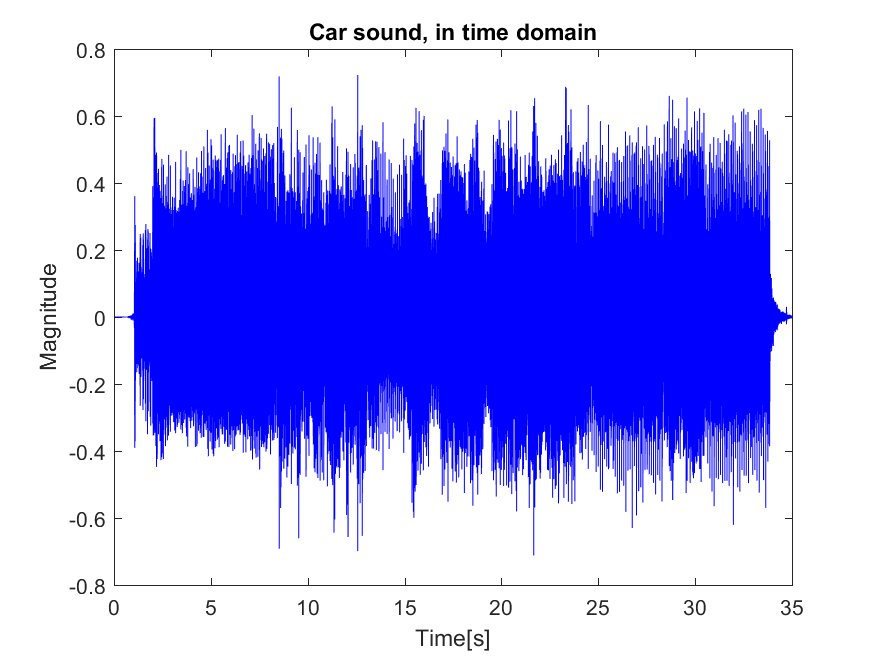
\includegraphics[width=\textwidth]{code/Car_figure1.png}
	\caption{kage}
	\label{fig:Car_figure1:1}
\end{figure}

\subsubsection{DFT}
\begin{figure}
	\centering
	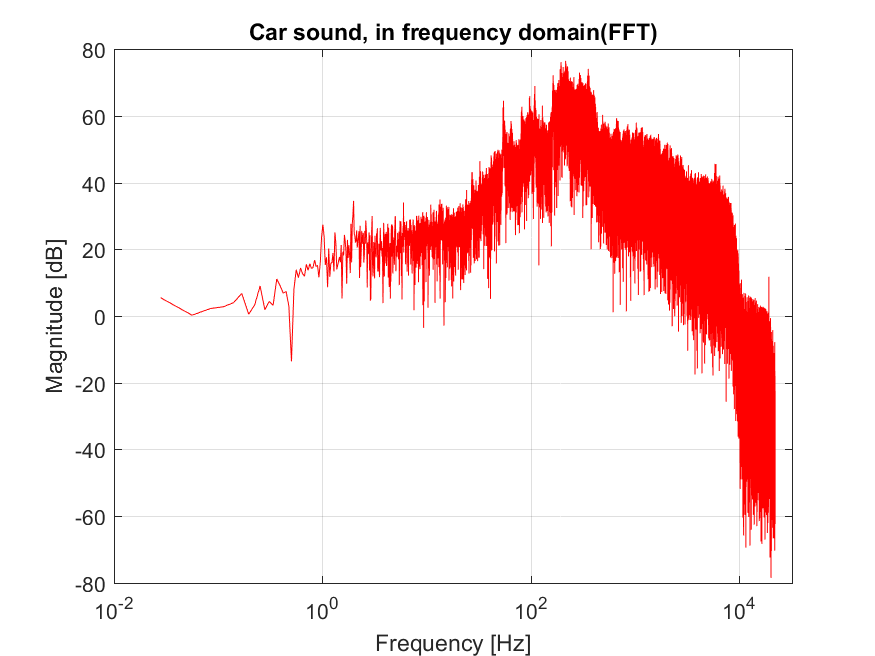
\includegraphics[width=\textwidth]{code/Car_figure2.png}
	\caption{}
	\label{fig:Car_figure2:2}
\end{figure}




\subsubsection{Analysis}



\subsubsection{Conclusion}

\subsection{Noise from a windmill}
\subsubsection{DFT}

\subsubsection{Analysis}

\subsubsection{Conclusion}

\subsection{EKG}
\subsubsection{DFT}

\subsubsection{Analysis}

\subsubsection{Conclusion}

\subsection{Breaking wine glass}
\subsubsection{DFT}

\subsubsection{Analysis}

\subsubsection{Conclusion}

\subsection{Music}
\subsubsection{DFT}

\subsubsection{Analysis}

\paragraph{Genre 1}

\paragraph{Genre 2}

\paragraph{Genre 3}

\paragraph{Genre 4}

\subsubsection{Conclusion}

\section{Further analysis of signals}
\label{sec:analysisOfSignals}
Eksperimenter med udglatning, zero-padding og windowing 